\documentclass[12pt,twoside]{ord}

%*******************AMS-latex*************
\usepackage{amssymb}
\usepackage{amsmath}     
%\usepackage{amsthm} %Do not use
%*********************************************** 
\usepackage{algorithmic} %style for algorithms
\usepackage[T1]{fontenc}
%****************************
%\usepackage{pdflscape} %style for lanscape page
\usepackage[]{algorithm2e}%a another possibe style for writing algortithms

\usepackage{lineno}	%package for proofs
%style for pre-proof version, do not uncomment this
%\usepackage{draftwatermark}
%\SetWatermarkText{Pre-proof}
%\SetWatermarkScale{0.5}



%Assigned by authors
%Titlte
\ORDtitle{Applications of robust optimization models to portfolio selection problem}
%Short authors
\ORDshortafill{J. Nowak et al.}
%Short title
\ORDshorttitle{Applications of robust optimization...}
%Authors affiliations (up to 4 affiliations, leave empty if not used}
\ORDaffilone{Department of Mathematics,Wroclaw University of Science and Technology, Wroclaw, Poland}
\ORDaffiltwo{Department of Computer Science, Faculty of Mathematical Sciences, University of Warsaw, Warsaw, Poland}
\ORDaffilthree{Department of Applied Mathematics, Poznan University, Poznan, Poland}
\ORDaffilfour{}
%Adding authors {<Name~Surname>}{<Id_affil>}{<Id_orcid>}{<E-mail>}
%You can add up to five authors. Leave empty if not used
\ORDauthorone{Jan~Nowak}{1}{000-000200-1}{}
\ORDauthortwo{Edward~Kowalski}{*1}{000-000200-2}{}
\ORDauthorthree{Joanna~Nowakowska}{2}{000-000200-3}{}
\ORDauthorfour{Marta~Kowalska}{3}{000-000200-4}{}
\ORDauthorfive{}{}{}{}
%Corresponding author e-mail
\ORDcorrespoding{$^*$Corresponding author, email address:}{e.kowalski@hnet.xxx}


%-------------------------------------------
%To be assigned by editors, do not edit this section
\ORDnumber{x}
\ORDvolume{xx}
\ORDdoi{DOI: draft}
\ORDyear{xxxx}
\ORDReceived{xxxxx~xxxxx}
\ORDRevised{xxxxx~xxxxx}
\ORDAccepted{xxxxx~xxxxx}
\ORDPublished{xxxxx~xxxxx}
\ORDFirstpagenum{1}
\ORDFounding{}
%-------------------------------------------

\begin{document}

\maketitle

%Provide abstract
\begin{abstract}
	The  abstract of about 150 words describing the main problems, results and conclusions presented in the paper. The  abstract of about 150 words describing the main problems, results and conclusions presented in the paper. The  abstract of about 150 words describing the main problems, results and conclusions presented in the paper. The  abstract of about 150 words describing the main problems, results and conclusions presented in the paper. The  abstract of about 150 words describing the main problems, results and conclusions presented in the paper. 
\end{abstract}

%Provide keywords

\ORDKeywords{keyword 1, keyword 2, keyword 3, keyword 4, keyword 5}
%\linenumbers % do not switch this

%Provide content of the paper
\section{Introduction}
\label{secintr}

\emph{Robust optimization} is a field of optimization theory that deals with optimization problems in which a certain measure of robustness is sought against uncertainty that can be represented as deterministic variability in the value of the parameters of the problem itself and/or its solution~\cite{BTN98}. A comprehensive description of robust optimization can be found in the book by Ben-Tal et al.~\cite{BGN09}. Other reference~\cite{K93}. 

Provide only necessary references. The number of references for non-survey papers should not exceed~$35$. For survey papers it may be larger. \textbf{The references should be provided in a separate BibTex file.} Please, verify carefully the correctness of all data in the references.

The paper is organized as follows. In Section~\ref{sec1}, we show...

\section{Problem formulation}
\label{sec1}



\begin{definition}[\cite{BGN09}]
\label{def1}
The robust optimization problem is defined as follows:
\begin{equation}
	\max_{\pmb{x}\in \mathbb{X}}\{f(\pmb{x}):\; g(\pmb{x},\pmb{u})\leq \pmb{b}\; \forall \pmb{u}\in \mathbb{U}\}
\end{equation}
\end{definition}



\section{Solution algorithm}
\label{sec2}


 Figures should be inserted as correct eps files of high quality. All figures must be referenced (Figure~\ref{fig1}).

\begin{figure}[ht]
\centering 
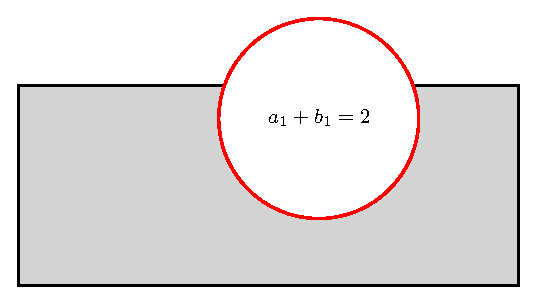
\includegraphics[scale=.8]{figure.eps}
\caption{A sample figure.}\label{fig1}
\end{figure}



\begin{lemma}
\label{lem1}
Write lemma here...
\end{lemma}
\begin{proof}
The proof of the lemma. We start by showing
\begin{equation}
\label{eq2}
	a^2+b^2=c^2
\end{equation}
It follows from~(\ref{eq2})...
\end{proof}

\begin{lemma}
\label{lem2}
Write lemma here...
\end{lemma}
\begin{proof}
The proof of the lemma....
\end{proof}

\begin{theorem} 
\label{thm1}
Write theorem here...
\end{theorem}
\begin{proof}
The proof of the theorem....
\end{proof}

\begin{corollary}
\label{cor1}
Write corollary here...
\end{corollary}

\begin{observation}
\label{obs1}
Write observation here...
\end{observation}

Write pseudocode of your algorithms using algorithm2e or algorithmic style.

\begin{algorithm}[h]
\KwIn {Array of integers $A=[a_1,\dots,a_n]$} 
\KwOut{The largest element in $A$}
$max:= a_1$\\
\For{$i:= 2$ \KwTo $n$} 
{ 
  \If{$a_i>max$} 
   {$max:= a_i$} 
} 
\textbf{return} $max$
\caption{Finding the largest element using algorithm2e.}\label{alg1}
\end{algorithm} 

\begin{algorithm}[h]
\begin{algorithmic}[1]
	\REQUIRE{Array of integers $A=[a_1,\dots,a_n]$}
	\ENSURE{The largest element in $A$}
	\STATE $max:=a_1$
	\FOR{$i:=1$ \textbf{to} $n$}
		\IF{$a_i>max$}
			\STATE $max:=a_i$
		\ENDIF
	\ENDFOR
\caption{Finding the largest element using algorithmic.}
\end{algorithmic}

\end{algorithm}


\subsection{Special case}
\label{subsec1}

In this section we consider...

\begin{theorem} 
\label{thm2}
Write theorem here...
\end{theorem}
\begin{proof}
The proof of the theorem....
\end{proof}

\subsubsection{Something else}

Write here something else...

\section{Computational tests}

All tables must be referenced (Table~\ref{tab1} and Table~\ref{tab2}). Big tables should fit to the size of the page. Very big table should be split into several smaller.

\begin{table}[h!]
\caption{The first table} \label{tab1}
\centering
\begin{tabular}{c|cccc} \hline
	Label 1 & Label 2 & Label 3 & Label 3 \\ \hline \hline
	 Steve & 23 & 33 & 12 \\
	 Adam & 3 & 3 & 12 \\
	 Ewa & 1 & & 23 \\ \hline
\end{tabular}
\end{table}



\begin{table}[h!]
\caption{The second table} \label{tab2}
\resizebox{17.5cm}{!} {
\begin{tabular}{c|ccccccccccccccccc} \hline
	Label 1 & Label 2 & Label 3 & Label 3 & Label 2 & Label 3 & Label 3 & Label 2 & Label 3 & Label 3 & Label 3 & Label 3 & Label 2 & Label 3 & Label 3 \\ \hline \hline
	 Steve & 23 & 33 & 12 & 23 & 33 & 12 & 23 & 33 & 12 & 23 & 33 & 12 & 12 & 12\\
	 Adam & 3 & 3 & 12& 23 & 33 & 12& 23 & 33 & 12& 23 & 33 & 12 & 12 & 12 \\
	 Ewa & 1 & & 23 & 23 & 33 & 12& 23 & 33 & 12&23 & 33 & 12 & 12 & 12\\ \hline
\end{tabular}
}
\end{table}




\section{Conclusions}
Write  your conclusions here.



\acknowledg{The authors are grateful to two anonymous reviewers for their valuable comments and suggestions made on the previous draft of this manuscript. This work has been supported by....}

\funding{First and Second author are supported by grant....}


\bibliographystyle{acm}
\bibliography{bibliography}


\appendix
\section{Appendix}
\label{appenA}
Write some additional proofs here... \footnote{aaa}
\section{Appendix}
\label{AppenB}
Write additional content here...

\end{document}